\documentclass[tikz,border=6mm]{standalone}
\usepackage{tikz}
\usepackage{xcolor}
\usetikzlibrary{arrows.meta,calc,decorations.pathmorphing,shapes.geometric,positioning,backgrounds,fit,shadings,patterns}
\definecolor{substblue}{RGB}{70,130,180}
\definecolor{procamber}{RGB}{180,110,30}
\definecolor{feltgreen}{RGB}{0,110,55}
\definecolor{bgcream}{RGB}{252,248,240}
\definecolor{atomblue}{RGB}{100,160,210}
\definecolor{emphred}{RGB}{160,40,40}
\definecolor{panelborder}{RGB}{180,170,155}

\begin{document}
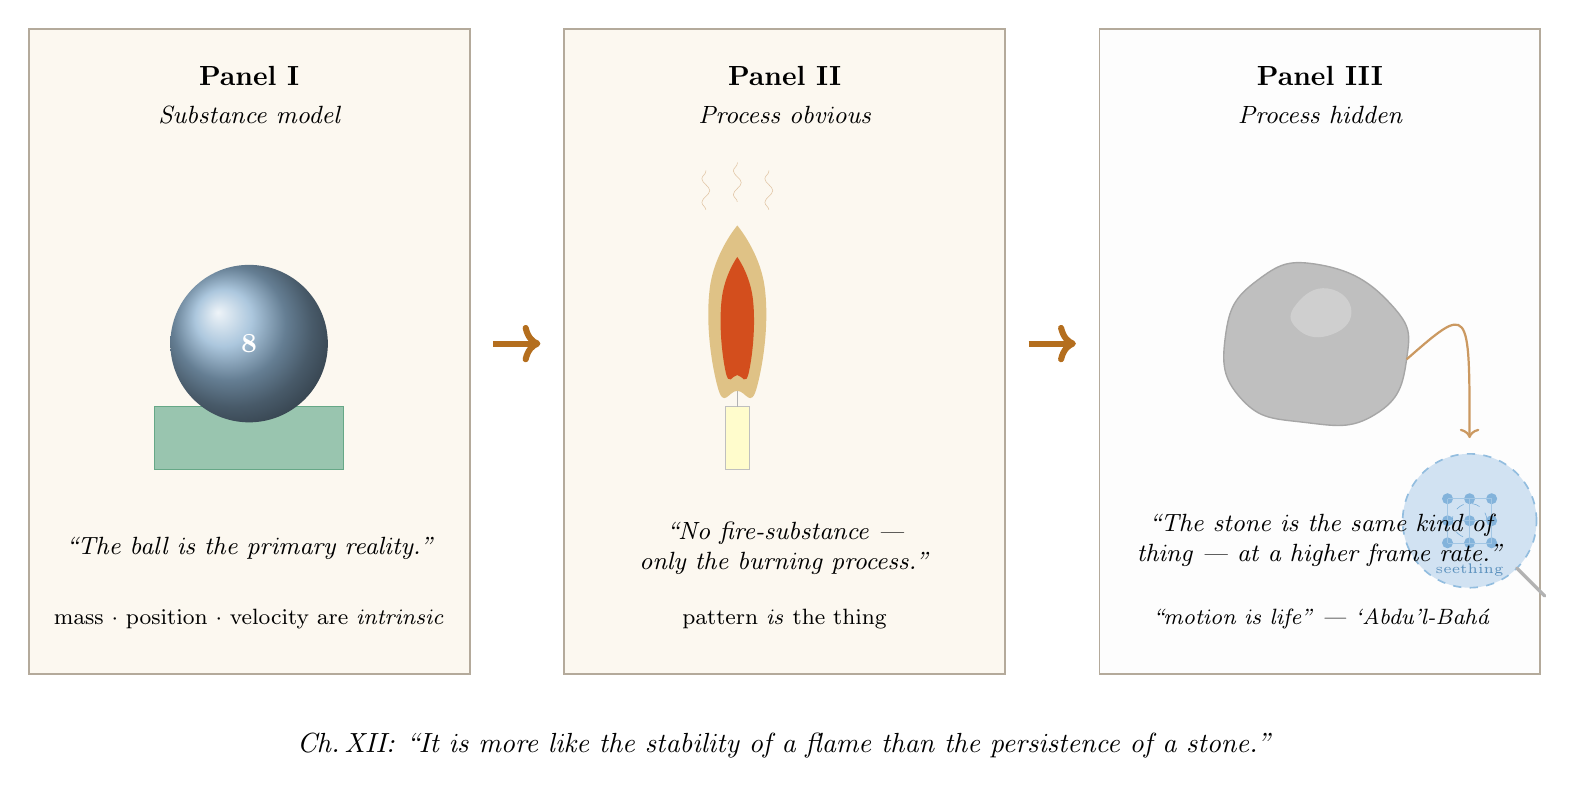
\begin{tikzpicture}[
  every node/.style={font=\sffamily},
  panel arrow/.style={->, very thick, procamber, line width=2.2pt},
]

% ===== Layout =====
% Three panels, each 5.6cm wide, gap 1.2cm for arrows
% Panel 1: x in [-9,  -3.4]
% Arrow 1:  x in [-3.4, -2.2]
% Panel 2: x in [-2.2,  3.4]
% Arrow 2:  x in [ 3.4,  4.6]
% Panel 3: x in [ 4.6, 10.2]
% y: -4.2 to 4.0, caption strip below

%% ============================================================
%% PANEL 1 — "The Substance Model"
%% ============================================================
\fill[bgcream, draw=panelborder, line width=0.7pt]
  (-9.0,-4.2) rectangle (-3.4, 4.0);

% Panel header
\node[font=\bfseries, align=center] at (-6.2, 3.4) {Panel I};
\node[font=\small\itshape, align=center] at (-6.2, 2.9) {Substance model};

% Green felt base
\fill[feltgreen!40, draw=feltgreen!60, line width=0.4pt]
  (-7.4,-1.6) rectangle (-5.0,-0.8);

% Billiard ball on felt
\shade[ball color=substblue!60!white] (-6.2,-0.0) circle (1.0cm);
\node[white, font=\bfseries] at (-6.2,-0.0) {8};

% Caption below
\node[font=\itshape\small, align=center] at (-6.2,-2.6)
  {``The ball is the primary reality.''};

% Small footer text
\node[font=\footnotesize, align=center] at (-6.2,-3.5)
  {mass $\cdot$ position $\cdot$ velocity are \emph{intrinsic}};

%% ============================================================
%% ARROW 1  (between panel 1 and panel 2)
%% ============================================================
\draw[panel arrow] (-3.1, 0) -- (-2.5, 0);

%% ============================================================
%% PANEL 2 — "Process Obvious"
%% ============================================================
\fill[bgcream, draw=panelborder, line width=0.7pt]
  (-2.2,-4.2) rectangle (3.4, 4.0);

% Panel header
\node[font=\bfseries, align=center] at (0.6, 3.4) {Panel II};
\node[font=\small\itshape, align=center] at (0.6, 2.9) {Process obvious};

% ----- Candle -----
% Candle body
\fill[yellow!20!white, draw=gray!50, line width=0.4pt]
  (-0.15,-1.6) rectangle (0.15,-0.8);

% Wick
\draw[gray!60, line width=0.5pt] (0,-0.8) -- (0,-0.6);

% Outer flame (teardrop: pointed at top, round at bottom)
\fill[procamber!80!yellow!60, opacity=0.85]
  plot[smooth, tension=0.8] coordinates {
    (0, 1.5)        % tip
    (0.35, 0.7)     % right bulge
    (0.25, -0.55)   % right base
    (0, -0.6)       % base center
    (-0.25,-0.55)   % left base
    (-0.35, 0.7)    % left bulge
    (0, 1.5)        % back to tip
  };

% Inner flame
\fill[procamber!60!red, opacity=0.90]
  plot[smooth, tension=0.8] coordinates {
    (0, 1.1)
    (0.20, 0.55)
    (0.15,-0.35)
    (0,-0.4)
    (-0.15,-0.35)
    (-0.20, 0.55)
    (0, 1.1)
  };

% Heat shimmer lines (short curved lines above flame)
\draw[procamber!40, very thin, decorate,
      decoration={snake, amplitude=0.5mm, segment length=3mm}]
  (-0.4, 1.7) -- (-0.4, 2.2);
\draw[procamber!40, very thin, decorate,
      decoration={snake, amplitude=0.5mm, segment length=3mm}]
  (0.0, 1.8) -- (0.0, 2.3);
\draw[procamber!40, very thin, decorate,
      decoration={snake, amplitude=0.5mm, segment length=3mm}]
  (0.4, 1.7) -- (0.4, 2.2);

% Caption
\node[font=\itshape\small, align=center] at (0.6,-2.6)
  {``No fire-substance ---\\only the burning process.''};

% Footer
\node[font=\footnotesize, align=center] at (0.6,-3.5)
  {pattern \emph{is} the thing};

%% ============================================================
%% ARROW 2
%% ============================================================
\draw[panel arrow] (3.7, 0) -- (4.3, 0);

%% ============================================================
%% PANEL 3 — "Process Hidden"
%% ============================================================
\fill[bgcream!90!atomblue!10, draw=panelborder, line width=0.7pt]
  (4.6,-4.2) rectangle (10.2, 4.0);

% Panel header
\node[font=\bfseries, align=center] at (7.4, 3.4) {Panel III};
\node[font=\small\itshape, align=center] at (7.4, 2.9) {Process hidden};

% Pebble / rounded stone shape
\fill[gray!50, draw=gray!70, line width=0.5pt]
  plot[smooth cycle, tension=0.85] coordinates {
    (7.4,  1.0)    % top
    (8.3,  0.5)    % right-top
    (8.5, -0.2)    % right
    (8.1, -0.9)    % right-bottom
    (7.2, -1.0)    % bottom
    (6.4, -0.7)    % left-bottom
    (6.2,  0.1)    % left
    (6.6,  0.8)    % left-top
  };
% Slight highlight
\fill[white, opacity=0.25]
  plot[smooth cycle, tension=0.9] coordinates {
    (7.1, 0.5)
    (7.5, 0.7)
    (7.8, 0.4)
    (7.5, 0.1)
    (7.1, 0.2)
  };

% Curved arrow from stone toward magnifying glass inset
\draw[->, thick, procamber!70,
      shorten >=2mm]
  (8.5,-0.2) .. controls (9.3, 0.5) .. (9.3,-1.4);

% Magnifying-glass inset (dashed circle, lower-right of panel)
\filldraw[fill=atomblue!30, draw=atomblue!70, dashed, line width=0.6pt]
  (9.3,-2.25) circle (0.85cm);

% Handle of magnifying glass
\draw[gray!60, line width=1.2pt, line cap=round]
  ({9.3+0.85*cos(-45)},{-2.25+0.85*sin(-45)}) --
  ({9.3+1.35*cos(-45)},{-2.25+1.35*sin(-45)});

% 3x3 grid of atoms inside inset
\foreach \ax in {-0.28, 0, 0.28} {
  \foreach \ay in {-0.28, 0, 0.28} {
    \fill[atomblue!80] ({9.3+\ax},{-2.25+\ay}) circle (0.07cm);
  }
}
% Bonds (horizontal and vertical nearest-neighbor lines)
\foreach \ax in {-0.28, 0} {
  \foreach \ay in {-0.28, 0, 0.28} {
    \draw[atomblue!60, very thin] ({9.3+\ax},{-2.25+\ay}) -- ({9.3+\ax+0.28},{-2.25+\ay});
  }
}
\foreach \ax in {-0.28, 0, 0.28} {
  \foreach \ay in {-0.28, 0} {
    \draw[atomblue!60, very thin] ({9.3+\ax},{-2.25+\ay}) -- ({9.3+\ax},{-2.25+\ay+0.28});
  }
}
% Small dashed orbital arc on center atom
\draw[atomblue!90, dashed, very thin]
  (9.3,-2.25) ++(0.22,0) arc (0:270:0.22cm);

% "seething" label inside inset
\node[font=\tiny, align=center, text=atomblue!90!black] at (9.3,-2.88)
  {seething};

% Caption
\node[font=\itshape\small, align=center] at (7.4,-2.5)
  {``The stone is the same kind of\\thing --- at a higher frame rate.''};

% Footer
\node[font=\footnotesize\itshape, align=center] at (7.4,-3.5)
  {``motion is life'' --- `Abdu'l-Bah\'a};

%% ============================================================
%% BOTTOM CAPTION (below entire figure)
%% ============================================================
\node[font=\itshape, align=center] at (0.6,-5.1)
  {Ch.\,XII: ``It is more like the stability of a flame than the persistence of a stone.''};

\end{tikzpicture}
\end{document}
